% !Mode:: "TeX:UTF-8"

\BiChapter{模型介绍}{}

\BiSection{环形动力学介绍}{}
环形结构在自然科学中极为常见,在生化系统中,系统完成封闭的环形运动,标志着生物活动的进行。下面通过酶促反应的例子,理解环形结构和环形动力学在生化系统中的重要作用。
\begin{equation*}
    E + S \xrightleftharpoons[k_{-1}]{k^{'}_1}
    ES \xrightleftharpoons[k_{-2}]{k^{'}_2}
    EP \xrightleftharpoons[k_{-3}]{k^{'}_3}
    E + P
\end{equation*}

上面的公式是酶促(Michaelis-Menten)反应方程,其中E是一个酶分子,反应物S在它的催化作用下生成产物P。追踪单个酶分子,它有三种状态:结合态ES,EP和自由态E,并持续在三者间转化。从时间维度,可以把酶状态的变化过程建模为三状态连续时间马氏链。酶分子在方程最左面的状态,和方程最右面的状态相同,因此该系统具有明显的环形结构。沿着该反应的正(反)方向会形成正(反)向环,这也对应了酶催化反应物S(产物P)转变为产物P(反应物S)的过程。

从上面例子可以看出,研究系统中的环结构和环形动力学是十分必要的。环形动力学理论的发展与非平衡态统计物理的发展是紧密相连的。其中的平衡态热力学是研究与外界没有能量和物质交换的系统,这对应于细致平衡条件下的马氏链。由于细致平衡下的马氏链是可逆的,因此可以用可逆马氏链对平衡态热力学系统建模。上个世纪初, Wegscheider 给出了化学反应系统处于细致平衡的充要条件,称为Wegscheider条件。后来,Kolmogorov从马氏链的角度给出了类似于该条件的命题,称为 Kolmogorov 环条件。该条件从数学层面严格证明出,如果平稳马氏链的任意环,沿着正向环的转移概率乘积与反向环的相等,那么它是可逆的。Kolmogorov环条件巧妙地把非平衡态统计物理的概念转化为环动力学的数学命题,这是一个重大的进步。大偏差和涨落定理都是非平衡态统计物理的重要概念,本文正是通过环流理论,解析它们的数学结构和物理内涵。

\BiSection{马氏链中的环}{}
本文通过离散时间马氏链$\xi = (\xi_n)_{n \ge 0}$对随机热力学系统建模,该模型的状态空间是$S = \{1, \dots N\}$,转移概率矩阵是$P=(p_{ij})_{i,j \in S}$,从状态$i$到状态$j$的转移概率为$p_{ij}$。记该马氏链对应的转移图为$G=(S, E)$,顶点集是状态空间$S$,有向边集是所有正转移概率的边$E$ \ref{figure:transitiongraph}。令$\langle i, j\rangle$表示状态$i$到状态$j$的有向边,因此有$E = \{\langle \langle i, j\rangle \in S \times S: p_{ij}>0\}$,且记$|E| = M$集合$E$中元素的数量。本文所考虑的马氏链都是不可约的,也就是有向图$G$是连通的。因此对某个状态,图$G$不仅包含其他状态流入的边,还包含到其自身的边,也就是一元环 \ref{figure:transitiongraph}。

图\ref{figure:transitiongraph}(c)所示的图拓扑是转移图$G$中的特殊情形,以往的研究中称该系统为单环马氏链。具体来说,如果马氏链$\xi$满足 $p_{ij}=0$且$|i-j| \ge 2$(其中的$i,j$是模$N$运算后的结果),则称为单环马氏链。单环系统在生物学方面具有特殊的意义,许多重要的生化过程,如酶和离子通道的构象变化\cite{cornish2013fundamentals,sakmann2013single},磷酸化-磷酸化循环\cite{beard2008chemical},甲基化-去甲基化循环\cite{jia2017nonequilibrium},以及染色体重塑导致的启动子的激活\cite{pedraza2008effects,jia2022analytical}都可以被建模为单环马氏链。下文中,重点关注单环系统,大部分的结论也可以扩展到一般系统。

\begin{figure}[h]\label{figure:transitiongraph}
\centering
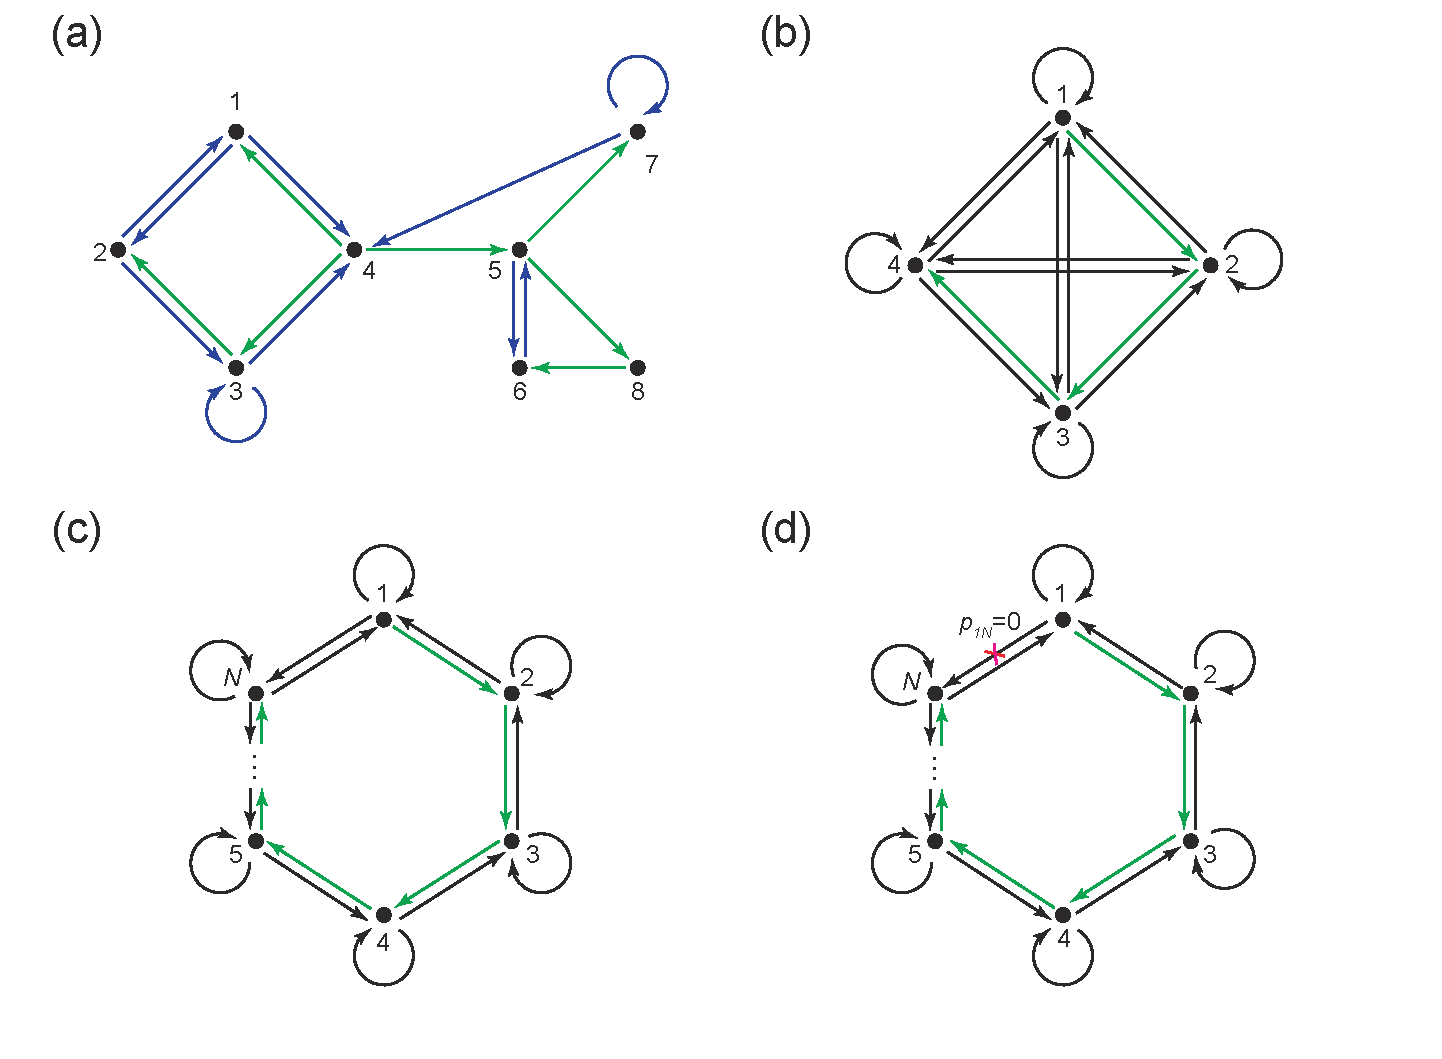
\includegraphics[scale=0.5]{chart/transitiongraph.pdf}
\caption{各类马氏链的转移图和相应的生成树 (a) 一般转移图的马氏链, 绿色线表示根节点为4的生成树$T$,并且蓝色线表示$T$的弦 (b) 四状态全连接马氏链,其中每个状态可以转移到自己和其他状态 (c) 
$N$状态单环马氏链。系统有一个环拓扑。每个状态转移到自身和它两个相邻节点 (d) 一个N状态的单环马尔科夫链,该系统无法从状态$1$转移到状态$N$ (b)-(d)中,绿色箭头表示生成树T}
\end{figure}

\BiSection{环擦除方式定义的环流}{}
本文主要研究和比较了马氏链中两种类型的环流,这个章节回顾环擦除方式定义的环流\cite{jiang2004mathematical,kalpazidou2007cycle}。马氏链中的回路是一个起点和终点相同的路径,比如路径$i_1 \to i_2 \to\cdots\to i_s \to i_1$(其中$i_1, i_2 , \cdots, i_s$是顶点集合$S$中不同点),其中$p_{i_1i_2}p_{i_2i_3}\cdots p_{i_si_1}>0$。若$j_1 \to j_2 \to\cdots\to j_r \to j_1$为另一个回路,两个回路等价,则是存在一个整数$k$且$r=s$,使得
\begin{equation*}
    j_1 = i_{k+1},j_2 = i_{k+2},\cdots,j_n = i_{k+s},
\end{equation*}
成立,其中指标$k+1,k+2,\cdots,k+s$为模$n$后的结果。在上述等价关系下,所有与回路$i_1 \to i_2 \to\cdots\to i_s \to i_1$等价的回路构成一个等价类,在此成为环$c = (i_1,i_2,\cdots,i_s)$。例如,$(1,2,3)$,$(2,3,1)$和$(3,1,2)$表示相同的环,且令环$(i_1,i_2,\cdots,i_s)$的反环为$(i_1,i_s,\cdots,i_2)$。系统中所有环的集合称为环空间$\mathcal{C}$。

马氏链轨道的会不断形成各种类型的环。如果持续去除马氏链$\xi$中的环,并且持续关注轨道中剩余的轨道,那么将会获得一个新的马氏链$\tilde{\xi} = (\tilde{\xi}_n)_{n\geq 0}$,称其为导出链。例如,最初的马氏链$\xi$的轨道为$\{1,2,3,3,2,3,4,1,4,\cdots\}$,相应的导出链$\tilde{\xi}$的变化过程和轨迹中形成的环为表 \ref{trajectory}所示。
\begin{table}[htb!]
    \renewcommand\arraystretch{1}\centering
    \begin{tabular}{cccccccccc} \hline\hline
   $n$            & 0 & 1 & 2 & 3   & 4     & 5 & 6 & 7         & 8 \\ \hline
   $\xi_n$         & 1 & 2 & 3 & 3   & 2     & 3 & 4 & 1         & 4 \\ \hline
   $\tilde{\xi}_n$& {[}1{]} & {[}1,2{]} & {[}1,2,3{]} & {[}1,2,3{]} & {[}1,2{]} & {[}1,2,3{]} & {[}1,2,3,4{]} & {[}1{]} & {[}1,4{]} \\ \hline
    \text{形成的环} &   &   &   & (3) & (2,3) &   &   & (1,2,3,4) &   \\ \hline\hline
    \end{tabular}
    \caption{导出链的变化过程和轨道中形成的环}\label{trajectory}
\end{table}

更为准确地说,导出链的状态是$S$的中不同状态组成的有限序列,一般记为$[i_1,i_2,\cdots,i_s]$。下面假设$\tilde{\xi}_{n-1}=[i_1,i_2,\cdots,i_s]$且$\xi_n = i_{s+1}$。若$i_{s+1}$不同于$i_1,i_2,\cdots,i_s$中任意一个,那么$\tilde{\xi}_n$就是$\tilde{\xi}_n = [i_1,i_2,\cdots,i_s,i_{s+1}]$。其次,若$i_{n+1}=i_r, \forall 1 \le r\le s$,那么$\tilde{\xi}_n$则是$\tilde{\xi}_n = [i_1,i_2,\cdots,i_r]$。对于该情况,称马氏链在时刻$n$形成环$(i_r,i_{r+1},\cdots,i_s)$。令$N^c_n$为环$c$在时刻$n$时总共形成的次数。那么可以定义环$c$在$n$时刻的经验环流:
\begin{equation*}
    J_n^c = \frac{1}{n}N^c_n,
\end{equation*}
相应的,$n$时刻经验净环流为:
\begin{equation*}
    \tilde{J}^c_n = J^c_n-J^{c-}_n.
\end{equation*}
更直观地看,$J^c_n$表示环$c$单位时间形成的数量,$\tilde{J}^c$表示环$c$单位时间形成的净数量。多数相关成果只研究了净环流的性质 \cite{Schnakenberg1976NetworkTO,andrieux2007fluctuation,andrieux2007network},本文还会进一步考虑环流的性质。

若令$n \to \infty$,那么经验环流$J^c_n$和 经验净环流$\tilde{J}^c$分别以概率为 1 趋近于$J^c$和$\tilde{J}^c$。极限$J^c$和$\tilde{J}^c$分别为环$c$的环流和净环流。关于$J^c_n$和$\tilde{J}^c$更为细致的叙述,可参考文献 \cite{jiang2004mathematical}。著名的环流分解定理 \cite{jiang2004mathematical} 可以通过上述定义写为:
\begin{equation}\label{decomposition}
    \pi_ip_{ij} = \sum_{c\ni\langle i,j\rangle}J^c,
\end{equation}
其中求和项考虑到了所有经过边 $\langle i, j\rangle$ 的环 $c$(符号 $c \ni \langle i, j\rangle$表示环$c$经过边$\langle i, j\rangle$),这也说明任意状态对的概率流可以分解为环流的和。

\BiSection{生成树方式定义的环流}{}
环流还可以通过生成树方式定义\cite{Schnakenberg1976NetworkTO,kalpazidou2007cycle}。记$T$为转移图$G$的有向子图,即$T$的所有边也是$G$的边,$\bar{T}$表示与$T$对应的无向图。满足下列三个条件的$T$被称为图$G$的生成树(极大树):
\begin{itemize}
    \item $T$是$G$的覆盖子图,即$T$包含$G$的所有顶点。
    \item $\bar{T}$是连通的。
    \item $\bar{T}$没有回路,其中无向图的回路是顶点到自身的无向路径。
\end{itemize}

下文使用$T$来表示生成树和它的边的集合。一般情况,生成树的选择不是唯一的,一个图可能有许多不同的生成树。任何生成树$T$必须包含$G$的的所有顶点,因此必须有$N-1$条边(见图 \ref{figure:transitiongraph}中的绿色箭头)\cite{kalpazidou2007cycle}。

一般称有向边$l \notin T$为$T$的弦(见图 \ref{figure:transitiongraph}(a)中的蓝色箭头)。因为$|E|=M$且$|T|= N-1$,所以任意生成树$T$都有$M-N+1$个弦。由于$\bar{T}$是连通的且没有回路,如果添加一根弦$l$到$T$,会导致无向子图$\overline{T \cup \{l\}}$恰好有一条回路。记$c_l$是由此产生的环,并且和$l$保持同样的指向。例如图 \ref{figure:transitiongraph}(c) 中所示的系统,如果在生成树$T$中添加弦 $l=\langle 2,1 \rangle$(蓝色箭头所示),那么可以得到环 $c_l=(2,1,4,3)$。由由弦生成的环的集合$\mathcal{L} = \{c_l: l\in E\setminus T\}$被称为基本集。由于弦和基本集之间的一一对应关系,可以用$c_l$形成的次数定义通过弦$l$的次数。$c_l$在$n$时刻的经验环流定义为:
\begin{equation*}
    Q^{c_l}_n = \frac{1}{n}\sum_{i=1}^n1_{\{\langle\xi_{i-1},\xi_i\rangle=l\}}.
\end{equation*}
其中$Q^{c_l}_n$表示单位时间通过弦$l$的次数。环擦除方式对于任意类型的环都可以定义,生成树方式只能把定义局限在基本集中环的环流。

类似的,也可以用生成树方式定义净环流。为此假设转移概率满足$p_{ij}>0$,当且仅当$p_{ji}>0$,这保障了系统的熵增量是有限值\cite{Schnakenberg1976NetworkTO,jiang2004mathematical}。对于任意弦$l$,$c_l$在时刻$n$的净环流为:
\begin{equation*}
    \tilde{Q}^{c_l}_n=Q^{c_l}_n-Q^{c_l-}_n.
\end{equation*}
如果$c_l$是一元环或者二元环,那么$c_l = c_{l^-}$,因此$\tilde{Q}_n^{c_l}=0$。对于弦$l=\langle i,j \rangle$,如果$c_l$是三元环或者多元环(包含超过三个状态的环),那么$l^-=\langle j,i\rangle$也是一个弦,并且$c_{l^-}$恰好是由弦$l^-$生成的环。文献 \cite{Schnakenberg1976NetworkTO, andrieux2007fluctuation, andrieux2007network}中,净环流只针对有三个及以上状态的的环定义,本文参考\cite{kalpazidou2007cycle}中的定义,使得净环流的定义也考虑了一元环和二元环。

若$n \to \infty$, 则经验环流$Q_n^{c_l}$和经验净环流$\tilde{Q}_n^{c_l}$将会分别以概率$1$趋于$Q^{c_l}$和$\tilde{Q}^{c_l}$。极限$Q^{c_l}$和$\tilde{Q}^{c_l}$分别作为环$c$的环流与净环流。对于弦$l=\langle i,j \rangle$,依据马氏链的遍历性,可得$Q^{c_l} = \pi_i p_{ij}$成立。

\BiSection{两种类型环流的比较}{}
下面将简述两种类型环流的差异。为讨论过程清晰,下面称环擦除方式定义的环流称为LE环流,生成树方式定义的环流称为ST环流。易知LE环流是定义在整个环空间$\mathcal{C}$,然而ST环流仅是针对基本集$\mathcal{L}$中的环定义。从环动力学角度,LE环流相较于ST环流给出了更完整的描述。而且,由于生成树一般并不唯一,不同的生成树选择会对应不同的ST环流。相比之下,LE环流并不依赖生成树的选择。

自然会问到基本集$\mathcal{L}$的规模会比环空间$\mathcal{C}$小多少。每根弦对应集合$\mathcal{L}$唯一一个元素,因此有$|\mathcal{L}| = |E\setminus T| = M-N+1$,所以很难对$|\mathcal{C}|$给出统一的表达式。为了深入探索,下面讨论两个特殊的案例。首先考虑转移图是全连接的马氏链,即$p_{ij}>0, \forall i,j \in S$,如图 \ref{figure:transitiongraph}(b)。其中$k$元环的数量是$\frac{N (N-1) \cdots (N-K+2)(N-k+1)}{k}$,因此
\begin{equation*}
    |\mathcal{C}| = \sum_{k=1}^N\frac{N\cdots (N-k+1)}{k}.
\end{equation*}
特别的,当$N=4$时,有$|\mathcal{C}|=24$,环空间为:
\begin{align*}
    \mathcal{C} = \{&(1),(2),(3),(4),(1,2),(1,3),(1,4),(2,3),(2,4),(3,4),\\
    &(1,2,3),(1,2,4),(1,3,2),(1,3,4),(1,4,2),(1,4,3),(2,3,4),(2,4,3),\\
    &(1,2,3,4),(1,2,4,3),(1,3,2,4),(1,3,4,2),(1,4,2,3),(1,4,3,2)\}.
\end{align*}
若选定生成树$T = 1\to 2\to 3\to 4$,那么有$|\mathcal{L}|=13$,基本集为:
\begin{align*}
    \mathcal{L} = \{&(1),(2),(3),(4),(1,2),(2,3),(3,4)\\
    &(1,2,3),(1,3,2),(2,3,4),(2,4,3),(1,2,3,4),(1,4,3,2)\}.
\end{align*}
因此对于全连接系统,ST环流会比LE环流少很多。

接下来考虑单环马氏链 \ref{figure:transitiongraph}(c)。为了叙述清晰,假设任意相邻状态$i$和$j$都满足$p_{ii}>0$和$p_{ij}>0$。这里,$|\mathcal{C}| = 2N +2$,并且环空间为:
\begin{equation}\label{cycle_space}
    \mathcal{C} = \{(1),\cdots,(N),(1,2),\cdots,(N-1,N),(N,1),(1,2,\cdots,N),(1,N,\cdots,2)\}.
\end{equation}
其中前$N$个环是一元环。中间$N$个环是二元环,最后两个环是$N$元环。如果选定生成树$T = 1\to 2\to\cdots \to N$,那么有$|\mathcal{L}| = 2N + 1$,并且基本集是:
\begin{equation*}
    \mathcal{L} = \{(1),\cdots,(N),(1,2),\cdots,(N-1,N),(1,2,\cdots,N),(1,N,\cdots,2)\}.
\end{equation*}
对于单环系统,只有唯一一个环,也就是说$(N, 1)$在环空间$C$中,却没有在基本集$\mathcal{L}$中。

为了进一步理解LE经验环流$J_n^c$和ST经验环流$Q_n^{c_N}$的关系,下面假设周期边界条件,即$\xi_0 = \xi_1$,这也是文献\cite{den2000large}中的标准假设条件。基于该假设,对任意弦$l$,易得:
\begin{equation}\label{conversion}
    Q_n^{c_l} = \sum_{c\in\mathcal{C}}J^c_n1_{\{l\in c\}}.
\end{equation}
其中求和项考虑到了所有经过弦$l$的环$c$(符号$c \ni l$表明$c$经过状态$i$)。既然上述方程两边都表示弦$l$单位时间形成的次数,这说明了ST环流可以表示为LE环流的线性组合。
